\documentclass[a4paper]{article}

% --- PACKAGES ---
\usepackage{mathtools}
\usepackage{a4wide,amssymb,epsfig,latexsym,multicol,array,hhline,fancyhdr}
\usepackage{vntex}
\usepackage{float}
\usepackage{amsmath}
\usepackage{lastpage}
\usepackage[lined,boxed,commentsnumbered]{algorithm2e}
\usepackage{enumerate}
\usepackage{color}
\usepackage{graphicx}
\usepackage{tabularx, caption}
\usepackage{multirow}
\usepackage{rotating}
\usepackage{geometry}
\usepackage{setspace}
\usepackage{tikz}
\usepackage[tikz]{bclogo}
\usetikzlibrary{calc,arrows,snakes,backgrounds}
\usepackage{listings}
\usepackage{environ}
\usepackage{soul}
\usepackage{hyperref}
\usepackage{xcolor}

% --- STYLING & COLORS ---
\hypersetup{urlcolor=blue,linkcolor=black,citecolor=black,colorlinks=true}
\definecolor{backcolour}{rgb}{0.95,0.95,0.92}
\definecolor{codegreen}{rgb}{0,0.6,0}
\definecolor{codegray}{rgb}{0.5,0.5,0.5}
\definecolor{codepurple}{rgb}{0.58,0,0.82}

\sethlcolor{gray!20}
\newcommand{\code}[1]{\hl{\texttt{#1}}}

\lstdefinestyle{mystyle}{
    backgroundcolor=\color{backcolour},
    commentstyle=\color{codegreen},
    keywordstyle=\color{magenta},
    numberstyle=\tiny\color{codegray},
    stringstyle=\color{codepurple},
    basicstyle=\ttfamily\footnotesize,
    breakatwhitespace=false,
    breaklines=true,
    captionpos=b,
    keepspaces=true,
    numbers=left,
    numbersep=5pt,
    showspaces=false,
    showstringspaces=false,
    showtabs=false,
    tabsize=2
}
\lstset{style=mystyle}

% --- THEOREMS ---
\newtheorem{theorem}{{\bf Theorem}}
\newtheorem{property}{{\bf Property}}
\newtheorem{proposition}{{\bf Proposition}}
\newtheorem{corollary}[proposition]{{\bf Corollary}}
\newtheorem{lemma}[proposition]{{\bf Lemma}}

% --- HEADER & FOOTER ---
\setlength{\headheight}{40pt}
\pagestyle{fancy}
\fancyhead{}
\fancyhead[L]{
 \begin{tabular}{rl}
    \begin{picture}(25,15)(0,0)
    \put(0,-8){
\includegraphics[width=8mm, height=8mm]{hcmut.png}} % Replace with your logo
   \end{picture}&
  \begin{tabular}{l}
    \textbf{\bf \ttfamily TRƯỜNG ĐẠI HỌC BÁCH KHOA - DHQG-HCM}\\
    \textbf{\bf \ttfamily KHOA KHOA HỌC VÀ KỸ THUẬT MÁY TÍNH}
  \end{tabular}
 \end{tabular}
}
\fancyhead[R]{}
\fancyfoot{}
\fancyfoot[L]{\scriptsize \ttfamily ĐỒ HỌA MÁY TÍNH - BÀI TẬP LỚN - Học kỳ II Năm học 2025 - 2026}
\fancyfoot[R]{\scriptsize \ttfamily Trang {\thepage}/\pageref{LastPage}}
\renewcommand{\headrulewidth}{0.3pt}
\renewcommand{\footrulewidth}{0.3pt}

% --- CUSTOM BOXES ---
\NewEnviron{sourcecoderemark}[1]{
  \par\smallskip\noindent
  \begin{tikzpicture}
    \node[inner sep=0pt] (box) {\parbox[t]{\dimexpr\linewidth-3pt\relax}{%
      \begin{minipage}{.2\linewidth}
      \centering\tikz[scale=3]\node[scale=2]{\bccrayon};
      \end{minipage}%
      \begin{minipage}{.75\linewidth}
      \textbf{#1}\par\smallskip
      \BODY
      \end{minipage}\hfill}%
    };
    \draw[red!75!black,line width=3pt]
      ( $ (box.north east) + (-5pt,3pt) $ ) -- ( $ (box.north east) + (0,3pt) $ ) -- ( $ (box.south east) + (0,-3pt) $ ) -- + (-5pt,0);
    \draw[red!75!black,line width=3pt]
      ( $ (box.north west) + (5pt,3pt) $ ) -- ( $ (box.north west) + (0,3pt) $ ) -- ( $ (box.south west) + (0,-3pt) $ ) -- + (5pt,0);
  \end{tikzpicture}\par\smallskip%
}

\NewEnviron{myremark}[1]
  {\par\smallskip\noindent
  \begin{tikzpicture}
    \node[inner sep=0pt] (box) {\parbox[t]{\dimexpr\linewidth-3pt\relax}{%
      \begin{minipage}{.2\linewidth}
      \centering\tikz[scale=3]\node[scale=2,rotate=30]{\bclampe};
      \end{minipage}%
      \begin{minipage}{.75\linewidth}
      \textbf{#1}\par\smallskip
      \BODY
      \end{minipage}\hfill}%
    };
    \draw[yellow!80!black,line width=3pt]
      ( $ (box.north east) + (-5pt,3pt) $ ) -- ( $ (box.north east) + (0,3pt) $ ) -- ( $ (box.south east) + (0,-3pt) $ ) -- + (-5pt,0);
    \draw[yellow!80!black,line width=3pt]
      ( $ (box.north west) + (5pt,3pt) $ ) -- ( $ (box.north west) + (0,3pt) $ ) -- ( $ (box.south west) + (0,-3pt) $ ) -- + (5pt,0);
  \end{tikzpicture}\par\smallskip%
}

%%%%%

\begin{document}

% --- TITLE PAGE ---

%%%%%%%%%%%%%%%%%%%%%%%%%%%%%%%%%
%%%%%%%%%%%%%%%%%%%%%%%%%%%%%%%%%

\begin{titlepage}
\begin{center}
ĐẠI HỌC QUỐC GIA THÀNH PHỐ HỒ CHÍ MINH \\
TRƯỜNG ĐẠI HỌC BÁCH KHOA
\end{center}
\vspace{1cm}
\begin{figure}[h!]
\begin{center}

\includegraphics[width=3cm]{hcmut.png} % Replace with your logo
\end{center}
\end{figure}
\vspace{1cm}
\begin{center}
\begin{tabular}{c}
\multicolumn{1}{c}{\textbf{{\Large ĐỒ HỌA MÁY TÍNH}}}\\
~~\\
\hline
\\
\textbf{{\Huge BÀI TẬP LỚN}}\\
\\
\hline
\end{tabular}
\end{center}
\vspace{3cm}
\begin{table}[h]
\begin{tabular}{rrl}
\hspace{3 cm} & Giáo viên hướng dẫn: & TS. Lê Thành Sách \\
& Sinh viên: & Hồ Trọng Nghĩa - 2252526. \\
\end{tabular}
\end{table}
\vfill
\begin{center}
{\footnotesize TP. HỒ CHÍ MINH, THÁNG 4/2026}
\end{center}
\end{titlepage}

%\thispagestyle{empty}
\renewcommand{\contentsname}{Mục lục}
\newpage
\tableofcontents
\newpage

% --- MAIN CONTENT ---

%%%%%%%%%%%%%%%%%%%%%%%%%%%%%%%%%
%%%%%%%%%%%%%%%%%%%%%%%%%%%%%%%%%

\section{Tổng quan chủ đề}
\hspace{12pt}
Bài báo cáo này mô tả chi tiết về kiến trúc phần mềm, các thư viện được sử dụng, cũng như các tính năng chính của engine đồ họa 3D được xây dựng nhằm phục vụ cho Bài tập lớn môn Đồ họa Máy tính (Học kỳ II Năm học 2025 - 2026).

Đề tài yêu cầu xây dựng một hệ thống hiển thị (render) các cảnh hình học 2D và 3D sử dụng pipeline đồ họa lập trình được (modern OpenGL với GLSL). Bên cạnh đó, ứng dụng còn tích hợp các tính năng mô phỏng trực quan giải thuật tối ưu hóa (Stochastic Gradient Descent), trực quan hóa cấu trúc phân tử, và đặc biệt là hệ thống sinh ảnh tổng hợp (synthetic image generator) nhằm tạo bộ dữ liệu cho các bài toán thị giác máy tính như phát hiện đối tượng, phân đoạn (segmentation) và ước lượng độ sâu.

\section{Mô tả chung}
\hspace{12pt}
Ứng dụng cung cấp một không gian tương tác 3D toàn diện với các tính năng sau:

\begin{itemize}
  \item \textbf{Quản lý và thao tác đối tượng:} Hỗ trợ tải các mô hình 3D đa định dạng (\code{.glb}, \code{.obj}, \code{.ply}) và khởi tạo các khối hình học cơ bản (Cube, Icosphere, Torus,...). Cho phép người dùng tương tác trực tiếp trong không gian 3D qua hệ thống Gizmo (tịnh tiến, xoay) hoặc qua các thanh trượt trên giao diện.
  \item \textbf{Hệ thống Camera linh hoạt:} Ứng dụng tích hợp hệ thống Arcball Camera hỗ trợ các thao tác xoay (orbit), di chuyển (pan), thu phóng (zoom) và tự động tập trung (focus) vào một đối tượng đang được chọn trong cảnh.
  \item \textbf{Chiếu sáng và Vật liệu:} Sử dụng mô hình chiếu sáng dựa trên vật lý (PBR), cho phép tinh chỉnh các thông số vật liệu như Albedo, Roughness, Metallic. Hệ thống hỗ trợ ánh xạ texture và nhiều loại nguồn sáng khác nhau (Point Light, Directional Light).
  \item \textbf{Trực quan hóa Toán học và Thuật toán:}
  \begin{itemize}
    \item Dựng lưới bề mặt 3D theo thời gian thực dựa trên các biểu thức toán học do người dùng nhập vào.
    \item Mô phỏng quá trình tối ưu hóa của các thuật toán như Stochastic Gradient Descent (SGD) và Momentum trên các hàm mất mát kinh điển (như hàm Rosenbrock), hiển thị quỹ đạo di chuyển của các thuật toán theo thời gian thực.
  \end{itemize}
  \item \textbf{Sinh dữ liệu tổng hợp (Dataset Generation):} Cho phép chụp lại khung hình hiện tại để xuất thành các tập dữ liệu huấn luyện AI. Dữ liệu đầu ra bao gồm ảnh màu RGB, bản đồ độ sâu (depth map) và mặt nạ phân đoạn (segmentation mask).
\end{itemize}

\section{Các kỹ thuật và thư viện được sử dụng}
\hspace{12pt}
Hệ thống được phát triển hoàn toàn bằng ngôn ngữ Python (yêu cầu phiên bản 3.10 trở lên) kết hợp với các thư viện đồ họa và tính toán hiệu năng cao. Để đảm bảo hiệu suất render, tính ổn định trên đa nền tảng và khả năng mở rộng, ứng dụng áp dụng các kỹ thuật phần mềm tiên tiến và mô hình kiến trúc tách biệt dữ liệu - logic.

\subsection{Các thư viện và yêu cầu kỹ thuật}
\hspace{12pt}
\begin{itemize}
    \item \textbf{OpenGL và quản lý phiên bản}: 
    Hệ thống sử dụng \code{PyOpenGL} và \code{PyOpenGL-accelerate} để tương tác với API OpenGL. Ứng dụng tạo context OpenGL 4.5 để tương thích tối đa với các công cụ gỡ lỗi đồ họa chuyên sâu như RenderDoc, mặc dù tập lệnh thực thi vẫn nằm trong giới hạn tính năng của 3.3.
    \begin{myremark}{Về macOS}
    Hệ thống sẽ yêu cầu OpenGL 4.1 thay vì 4.5 nếu phát hiện macOS. Lớp \code{Shader} tự động thực hiện patch mã nguồn shader bằng regex tại thời điểm chạy (ví dụ: chuyển \code{\#version 450 core} thành \code{\#version 410 core}).
    \end{myremark}

    \item \textbf{Quản lý cửa sổ và giao diện}: \code{glfw} được sử dụng để khởi tạo window context và xử lý sự kiện đầu vào. Giao diện người dùng (UI) được xây dựng thông qua \code{imgui-bundle} (Dear ImGui), cung cấp các bảng điều khiển như Inspector và Scene Panel.

    \item \textbf{Tính toán và xử lý dữ liệu}: \code{numpy} đóng vai trò trung tâm trong việc thực hiện các phép toán ma trận/vector tốc độ cao, tính toán AABB (Axis-Aligned Bounding Box) trong thời gian thực và biên dịch các hàm toán học để tạo lưới bề mặt 3D.

    \item \textbf{Xử lý tài nguyên}: \code{trimesh} được sử dụng để phân tách biểu đồ phân cấp (scene graph) từ các định dạng \code{.glb, .gltf, .obj, .ply}. \code{Pillow} đảm nhiệm việc giải mã hình ảnh. Hệ thống tận dụng sRGB textures của OpenGL để tự động chuyển đổi gamma sang không gian màu tuyến tính (linear color space), đảm bảo tính nhất quán về ánh sáng.
\end{itemize}

\subsection{Kiến trúc Entity-Component-System (ECS)}
\hspace{12pt}
Thay vì sử dụng Lập trình hướng đối tượng (OOP) truyền thống, hệ thống được thiết kế theo kiến trúc \textbf{ECS (Entity-Component-System)}. Kiến trúc này phân tách hoàn toàn dữ liệu ra khỏi logic xử lý, giúp tăng tính linh hoạt và tối ưu hóa việc lặp qua hàng loạt đối tượng trong đồ họa máy tính. Trung tâm của kiến trúc này là \code{Registry} quản lý toàn bộ vòng đời của thực thể và thành phần.

\subsubsection{Thực thể (Entity) và Thành phần (Component)}
\hspace{12pt}
\textbf{Entity} là những định danh nhẹ đại diện bằng số nguyên (\code{int}). Hệ thống hỗ trợ quan hệ cha-con (parent-child relationship), cho phép thực hiện dọn dẹp phân cấp (\textit{hierarchical disposal}). Khi một Entity cha bị xóa, toàn bộ Entity con sẽ tự động được giải phóng để tránh rò rỉ bộ nhớ.

\textbf{Component} là các cấu trúc dữ liệu thuần túy (triển khai bằng \code{@dataclass}), định nghĩa thuộc tính của Entity:
\begin{itemize}
    \item \code{Transform}: Lưu trữ vị trí, tỷ lệ và phép quay. Sử dụng Quaternion để tránh hiện tượng khóa trục (Gimbal lock) và đảm bảo nội suy mượt mà.
    \item \code{Visuals}: Liên kết Entity với Mesh và Material; quản lý chế độ vẽ (Fill/Wireframe) và thiết lập culling mặt sau (back-face culling).
    \item \code{Material}: Lưu trữ các tham số PBR bao gồm Albedo, Roughness, Metallic, Reflectance và Ambient Occlusion (AO), hỗ trợ cả giá trị hằng số và bản đồ texture.
    \item \code{Camera}: Định nghĩa thông số phối cảnh như FOV và các mặt phẳng cắt (clipping planes).
    \item \code{PointLight} và \code{DirectionalLight}: Định nghĩa nguồn sáng điểm (có suy giảm theo khoảng cách) và nguồn sáng hướng (song song, mô phỏng ánh sáng mặt trời).
\end{itemize}

Ngoài ra, hệ thống sử dụng các \textbf{Thành phần Singleton} để quản lý trạng thái toàn cục:
\begin{itemize}
    \item \code{Disposal}: Danh sách Entity chờ giải phóng.
    \item \code{UiState}: Trạng thái điều hướng và Entity đang chọn.
    \item \code{CameraState}: Ma trận View/Projection và dữ liệu camera chính.
    \item \code{IconRenderState}: Cấu hình hiển thị biểu tượng trong viewport.
    \item \code{RenderState}: Quản lý handle FBO, texture, shader và dữ liệu bounding box.
    \item \code{AssetsState}: Quản lý thread pool, hàng đợi công việc và bộ nhớ đệm tài nguyên.
    \item \code{SpawnerState}: Yêu cầu khởi tạo Entity từ model đã nạp.
    \item \code{GizmoState}: Trạng thái tương tác và tính toán của hệ thống Gizmo.
\end{itemize}

\begin{sourcecoderemark}{Mã nguồn}
Mã nguồn chứa các Component nằm ở \code{src/entities/components}.
\end{sourcecoderemark}

\subsubsection{Hệ thống xử lý (System)}
\hspace{12pt}
\textbf{System} chứa logic nghiệp vụ, thực hiện các phép toán trên các Entity có Component tương ứng.

\begin{itemize}
    \item \textbf{AssetSystem}: Là hệ thống bất đồng bộ quản lý vòng đời model và texture. Để tránh làm treo luồng render chính, hệ thống sử dụng một luồng worker chạy ngầm theo dõi \code{task\_queue}. Khi yêu cầu tài nguyên, hệ thống trả về một proxy với trạng thái \code{AssetStatus.Loading}. Sau khi \code{trimesh} và \code{Pillow} xử lý xong, kết quả được đẩy vào \code{result\_queue} để luồng chính thực hiện các thao tác nhạy cảm với OpenGL (tạo VAO, VBO, mipmap). Hệ thống có cơ chế caching theo đường dẫn file và xử lý lỗi chi tiết để tránh crash ứng dụng.

    \item \textbf{RenderSystem}: Thực thi pipeline render 3D sử dụng \code{tf2\_ggx\_shader}. 
    \begin{itemize}
        \item \textit{Mô hình ánh sáng}: Áp dụng PBR nâng cao với thành phần \textit{Hammon visibility} và \textit{Hammon GGX diffuse} cho phản xạ gương và tán xạ bề mặt chính xác. \textbf{Chỉ có trên branch \code{master} cho Bài tập lớn 2. Bài tập lớn 1 ở branch \code{a1p1} chỉ có Phong, Gouraud và Flat.}
        \item \textit{Hậu xử lý}: Sử dụng \textit{AgX tonemapping} để xử lý màu sắc HDR và hiệu ứng film grain.
        \item \textit{Sinh dữ liệu}: Thực hiện pass render phụ với \code{id\_shader} ghi Entity ID vào framebuffer 32-bit unsigned integer (\code{R32UI}). Hệ thống đảm bảo các sub-mesh của một model phức tạp dùng chung ID cha để tạo mask phân đoạn nhất quán. Sau đó, sử dụng NumPy để kiếm các Entity không bị che trên mask, và ánh xạ Entity ID qua thể loại vật thể cho mask cuối. Cuối cùng, xuất đồng bộ ảnh RGB, depth map 16-bit, nhãn YOLO và segmentation mask.
    \end{itemize}

    \item \textbf{UiSystem}: Quản lý giao diện qua \code{imgui-bundle}. Điểm nổi bật là cơ chế đồng bộ hai chiều giữa góc Euler và Quaternion: khi người dùng chỉnh Euler, hệ thống tính toán hai Quaternion tiềm năng và dùng \textit{dot product} để chọn giá trị gần nhất, tránh hiện tượng "lật" hình. Đồng thời sử dụng hàm \code{minimize\_euler} để giữ giá trị trong khoảng $[-180^\circ, 180^\circ]$. Ngoài ra, hệ thống còn phối hợp với \code{AssetSystem} để tạo mesh xem trước (Sphere, Torus, Cube) theo thời gian thực trước khi thêm vào scene.

    \item \textbf{CameraSystem}: Triển khai logic \textit{Arcball Camera} (quay, tịnh tiến, thu phóng) và đồng bộ hóa vị trí camera với điểm tiêu điểm (focal point), cập nhật ma trận View/Projection vào \code{CameraState}.

    \item \textbf{GizmoSystem}: Cung cấp tay cầm tương tác 3D. Với phép tịnh tiến, hệ thống tính giao điểm của chuột với một mặt phẳng ảo song song với trục được chọn. Với phép quay, nó theo dõi delta góc của chuột so với tâm vật thể. Kích thước Gizmo được scale động theo khoảng cách đến camera để giữ nguyên kích cỡ trên màn hình.

    \item \textbf{SpawnerSystem}: Chịu trách nhiệm hiện thực hóa các asset đã nạp. Khi một model chuyển sang trạng thái \code{Ready}, hệ thống duyệt các node, tạo Entity tương ứng và gán các Component \code{Transform}, \code{Visuals}, \code{Material}, đồng thời chuyển đổi tọa độ cục bộ sang tọa độ thế giới.

    \item \textbf{IconRenderSystem}: Chiếu vị trí thế giới của các Entity "vô hình" (đèn, camera) lên màn hình 2D. Sử dụng background draw list của ImGui để vẽ các biểu tượng FontAwesome, giúp người dùng dễ dàng định vị và chọn đối tượng trong không gian.

    \item \textbf{DisposalSystem}: Quản lý việc xóa Entity an toàn. Hỗ trợ xóa đệ quy toàn bộ cây phân cấp trừ khi Entity được đánh dấu bằng \code{EntityFlags} đặc biệt.

    \item \textbf{TransformInheritanceSystem}: Cập nhật ma trận biến đổi dựa trên quan hệ cha-con, đảm bảo mọi biến đổi của vật thể cha được kế thừa chính xác bởi các vật thể con trong Scene Graph.
\end{itemize}

\subsection{Các hệ thống chuyên biệt}
\hspace{12pt}
Để phục vụ các bài tập lớn, hệ thống tích hợp thêm các module chuyên sâu:
\begin{itemize}
    \item \textbf{SceneGeneratorSystem}: Tự động tạo môi trường đường phố phức tạp dựa trên cấu hình \code{SceneGeneratorState} (kích thước đường, mật độ nhà cửa). Hệ thống gán các nhãn phân loại (\code{Vehicle}, \code{Building}) để phục vụ RenderSystem sinh label chính xác.
    \item \textbf{SceneAnimatorSystem}: Mô phỏng giao thông dựa trên luật: tính toán gia tốc/phanh dựa trên khoảng cách để tránh va chạm, thực hiện chuyển làn mượt mà với hiệu ứng nghiêng thân xe, và áp dụng \textit{world-wrapping} (vòng lặp thế giới) để duy trì luồng giao thông liên tục.
    \item \textbf{FunctionSurfaceSystem}: Phân tích các biểu thức toán học từ \code{SurfaceFunction} thông qua \code{numpy} để tạo lưới tam giác 3D. Hệ thống chỉ biên dịch lại mesh khi biểu thức hoặc tham số thay đổi.
    \item \textbf{GradientDescentSurfaceSystem}: Triển khai các thuật toán tối ưu hóa (SGD, Momentum) trên các hàm mất mát (ví dụ: Rosenbrock). Hệ thống cập nhật vị trí các Entity "Optimizer" theo gradient của bề mặt và ghi lại quỹ đạo để trực quan hóa.
\end{itemize}

\begin{sourcecoderemark}{Mã nguồn}
Mã nguồn chứa các System nằm ở \code{src/entities/systems}.
\end{sourcecoderemark}

%%%%%%%%%%%%%%%%%%%%%%%%
%%%%%%%%%%%%%%%%%%%%%%%%
%%%%%%%%%%%%%%%%%%%%%%%%

\section{Các tính năng đã thực hiện}
\hspace{12pt}
Hệ thống hoàn thiện hầu hết các yêu cầu đề ra trong cả hai bài tập lớn, cụ thể như sau:

\subsection{Bài tập lớn 1: Dựng hình và Trực quan hóa}
\hspace{12pt}
\begin{itemize}
  \item \textbf{Phần 1 - Vẽ các hình cơ bản:}
  \begin{itemize}
    \item Hiện thực đầy đủ các hình 2D (tam giác, hình chữ nhật, đa giác đều, hình tròn, elip, hình thang, ngôi sao, mũi tên) và các khối 3D (lập phương, mặt cầu, trụ, nón, xuyến, lăng trụ).
    \item Khối cầu được mô hình hóa qua 3 phương pháp: Chia nhỏ tứ diện, chiếu lưới vuông lên mặt cầu và sử dụng tọa độ kinh vĩ độ.
    \item Hỗ trợ nhiều chế độ hiển thị: \textbf{Chỉ có trên branch \code{a1p1} trên kho GitHub.} Màu phẳng (Flat), nội suy đỉnh (Gouraud), chiếu sáng theo điểm ảnh (Phong), texture mapping, và khung dây (Wireframe).
    \item Tích hợp hệ thống nhiều nguồn sáng và nhiều camera cho phép chuyển đổi và tương tác linh hoạt.
  \end{itemize}
  \item \textbf{Phần 2 - Mô phỏng Gradient Descent:}
  \begin{itemize}
    \item Trực quan hóa bề mặt (surface) và đường đồng mức (contour) của các hàm mất mát: Himmelblau, Rosenbrock, Booth và Quadratic.
    \item Cho phép chạy song song nhiều bộ tối ưu hóa với các giải thuật: SGD, Momentum, Adam.
    \item Người dùng có thể điều chỉnh trực tiếp các siêu tham số như learning rate, momentum và tốc độ mô phỏng ngay trong quá trình chạy, hay dùng gizmo để di chuyển optimizer.
  \end{itemize}
\end{itemize}

\subsection{Bài tập lớn 2: Bộ sinh ảnh tổng hợp}
\hspace{12pt}
Hệ thống được thiết kế để tạo ra các tập dữ liệu huấn luyện cho bài toán xe tự hành với các thành phần:
\begin{itemize}
  \item \textbf{Sinh dữ liệu đa tầng:} Xuất đồng thời ảnh RGB chất lượng cao, bản đồ độ sâu (depth map) và mặt nạ phân đoạn (segmentation mask) khớp hoàn toàn về độ phân giải.
  \item \textbf{Gán nhãn tự động:} Tự động tính toán và xuất nhãn hộp giới hạn (Bounding Box) theo định dạng YOLO.
  \item \textbf{Cấu hình cảnh:} Hệ thống tự động nạp các mô hình xe và môi trường từ file model kèm sẵn trong mã nguồn, cho phép ngẫu nhiên hóa vị trí, kèm theo đó thay đổi góc nhìn và nguồn sáng (các tính năng đã có từ Bài tập lớn 1) để tăng tính đa dạng cho bộ dữ liệu.
\end{itemize}

\section{Hướng dẫn sử dụng}
\hspace{12pt}
Ứng dụng cung cấp giao diện trực quan giúp người dùng dễ dàng làm quen và thao tác.

\subsection{Điều khiển Camera và Quan sát}
\hspace{12pt}
\begin{itemize}
  \item \textbf{Xoay (Orbit):} Nhấn giữ và kéo \textbf{Chuột trái} để quay quanh điểm hội tụ.
  \item \textbf{Di chuyển (Pan):} Nhấn giữ \textbf{Chuột giữa} (hoặc con lăn) để di chuyển tịnh tiến camera.
  \item \textbf{Thu phóng (Zoom):} Sử dụng \textbf{Con lăn chuột} hoặc nhấn giữ \textbf{Chuột phải} để phóng to/thu nhỏ.
  \item \textbf{Tập trung (Focus):} Chọn một Entity trong danh sách và nhấn \code{Focus camera on this} để đặt tâm camera vào vật thể đó.
\end{itemize}

\subsection{Quản lý và Tương tác Vật thể}
\hspace{12pt}
\begin{itemize}
  \item \textbf{Thêm vật thể:} Sử dụng menu \code{+ Add} trong Scene Panel để chọn khối cơ bản hoặc tải mô hình từ file. Một bản xem trước (preview) màu xanh sẽ xuất hiện trước khi người dùng xác nhận thêm vào cảnh.
  \item \textbf{Gizmo trực quan:} Khi chọn một vật thể, hệ thống Gizmo sẽ xuất hiện. Người dùng có thể chuyển đổi giữa chế độ \code{Translate} (di chuyển theo trục) và \code{Rotate} (xoay quanh trục) ngay trên viewport.
  \item \textbf{Inspector:} Cho phép chỉnh sửa chi tiết các thông số về Transform, thuộc tính vật liệu (Albedo, Roughness, Metallic, Reflectance, AO) và thay đổi texture (Albedo, Normal, Roughness, Metallic) cho từng vật thể.
\end{itemize}

\subsection{Công cụ chuyên dụng}
\hspace{12pt}
\begin{itemize}
  \item \textbf{Hàm toán học (Bài tập lớn 1):} Thêm \code{Function surface}, nhập biểu thức vào trường \code{Expression} (ví dụ: \code{np.sin(x) * np.cos(z)}). Nhấn \code{Compile} để cập nhật hình dạng. Có thể sử dụng những hàm NumPy như \code{np.sin}, \code{np.cos}, v.v..
  \item \textbf{Sinh dữ liệu (Bài tập lớn 2):} Khi khởi động ứng dụng, sẽ mặc định tạo một Entity \textbf{Street scene}. Khi chọn Entity này, có thể tinh chỉnh cảnh trong phần \code{Inspector}, như các thông số ngẫu nhiên hóa cảnh trong Component \code{SceneGeneratorState} và chạy cảnh trong \code{SceneAnimatorState}. Trong phần \code{Graphics}, nhấn \code{Capture this frame} hoặc \code{Start multi-frame capture} để hệ thống tự động lưu ảnh RGB, nhãn phân đoạn và bản đồ độ sâu vào thư mục \code{dataset/}.
\end{itemize}

\section{Hình chụp màn hình}
\hspace{12pt}
\begin{figure}[H]
  \centering
  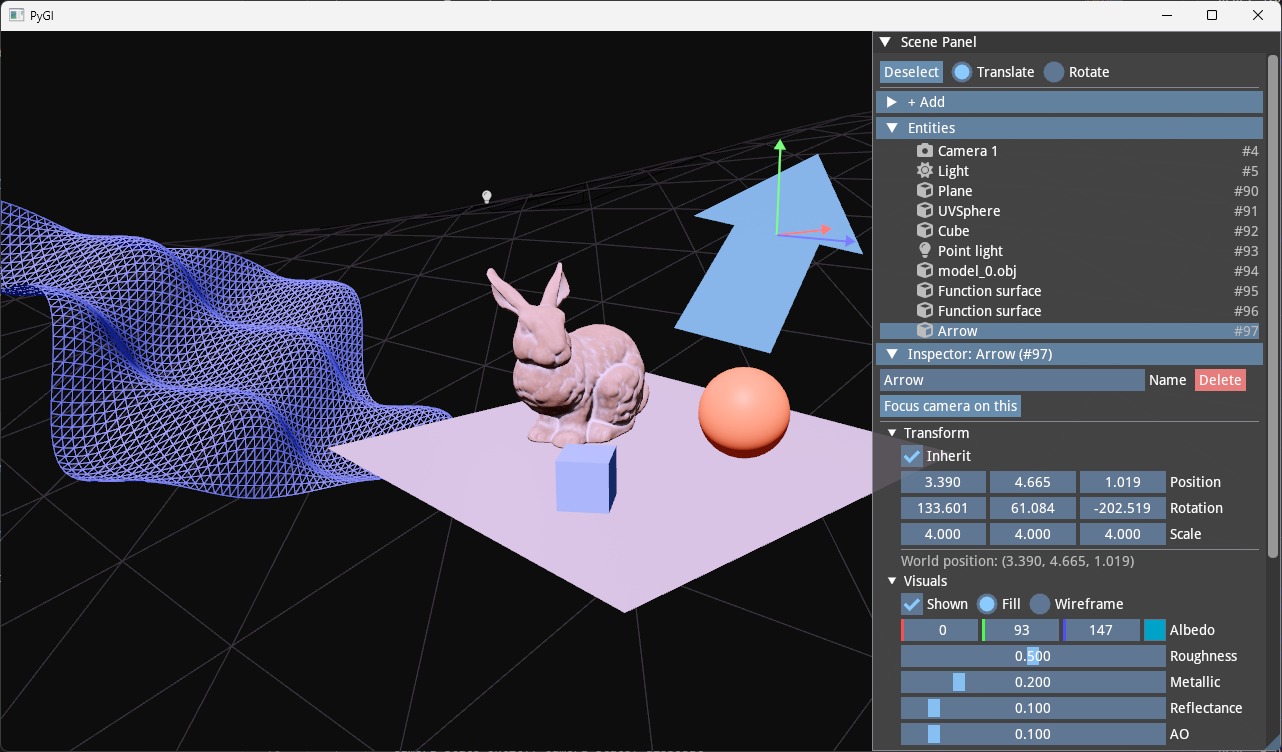
\includegraphics[scale = 0.4]{1777306072_ETMGw.png}
  \caption{Dựng ảnh (Bài tập lớn 1)}
\end{figure}

\begin{figure}[H]
  \centering
  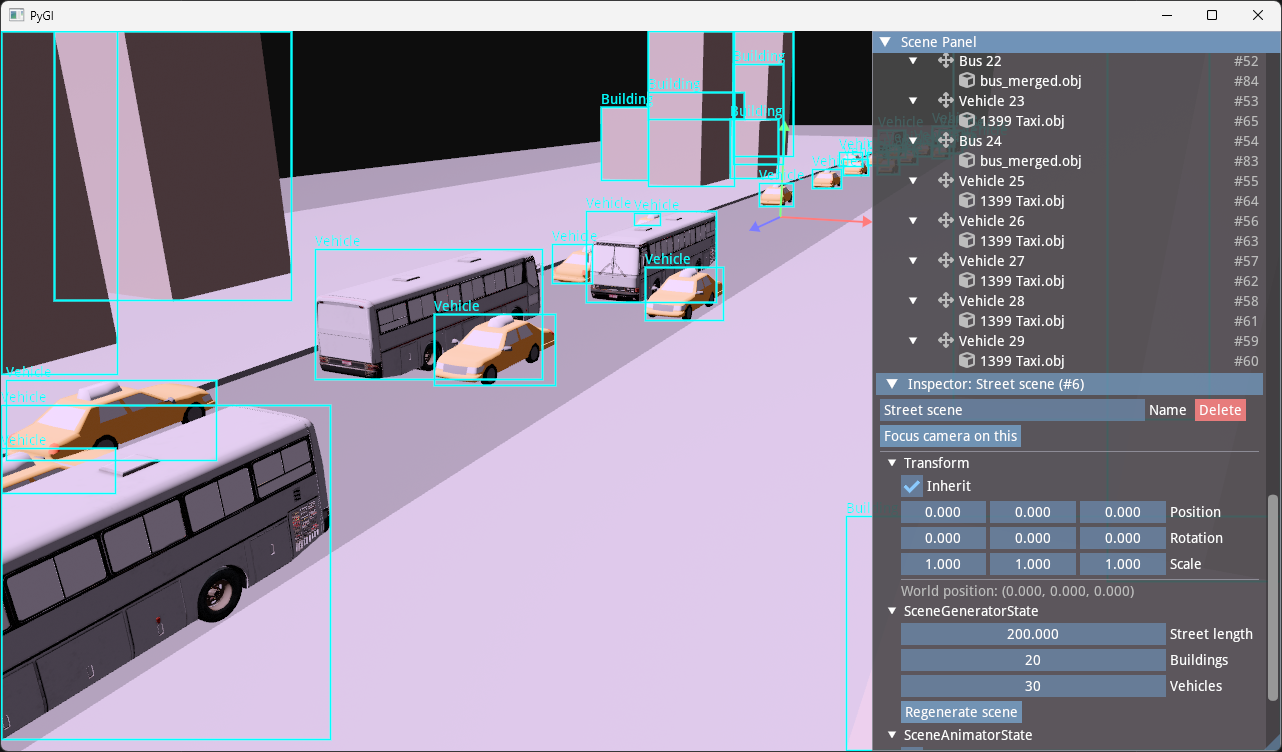
\includegraphics[scale = 0.4]{1777306552_fTv41.png}
  \caption{Dựng ảnh (Bài tập lớn 2)}
\end{figure}

\begin{figure}[H]
  \centering
  \begin{minipage}{0.32\textwidth}
    \centering
    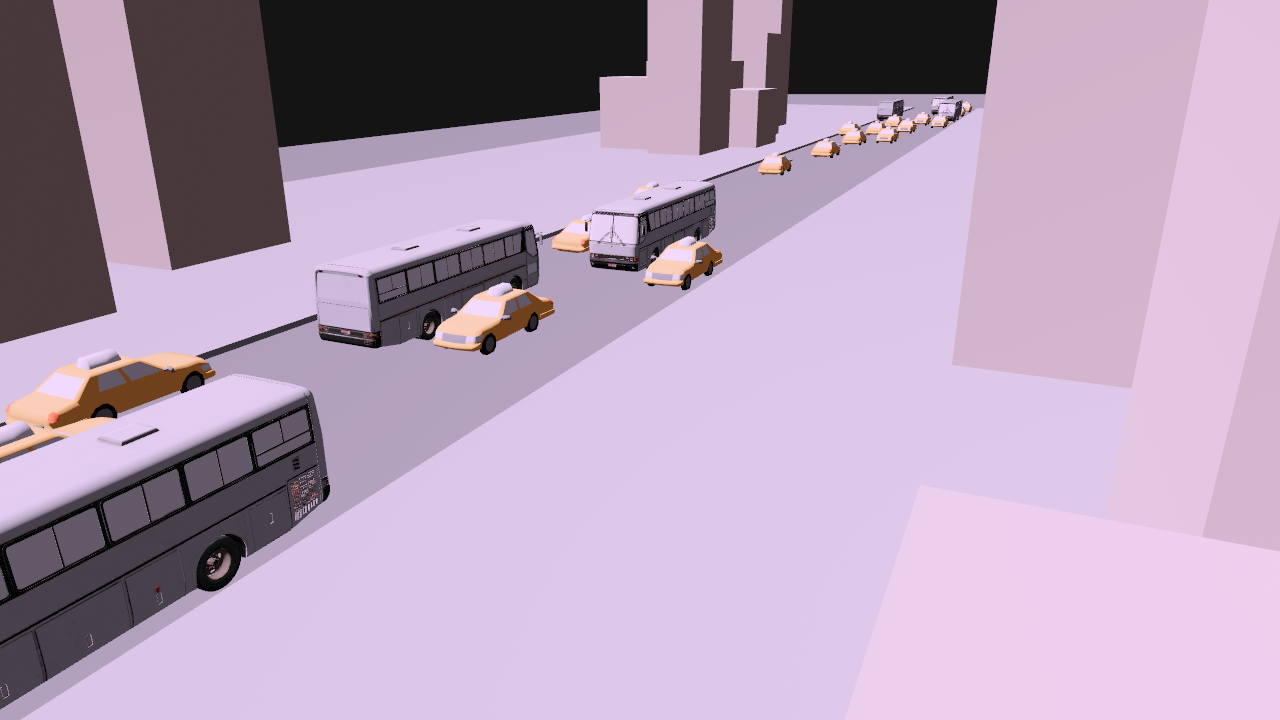
\includegraphics[width=\linewidth]{000000_rgb.png}
    \caption{Ảnh RGB}
  \end{minipage}\hfill
  \begin{minipage}{0.32\textwidth}
    \centering
    
\includegraphics[width=\linewidth]{000000_depth.png}
    \caption{Ảnh Depth}
  \end{minipage}\hfill
  \begin{minipage}{0.32\textwidth}
    \centering
    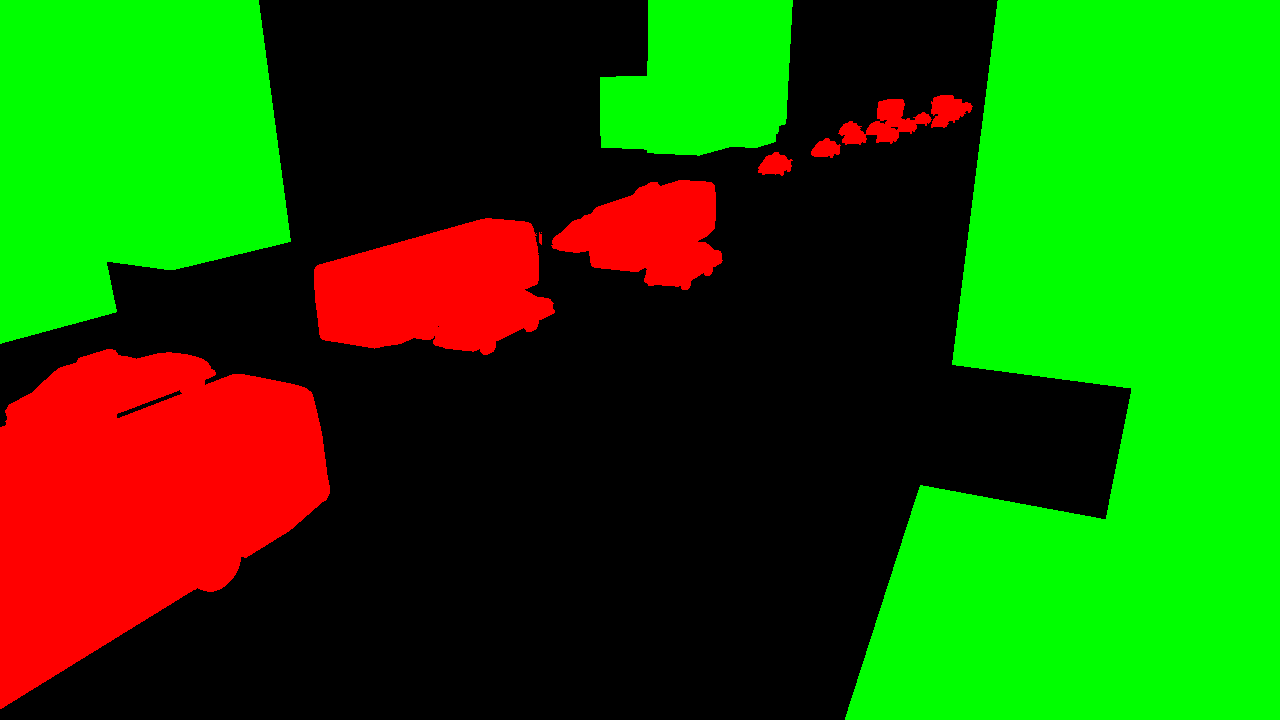
\includegraphics[width=\linewidth]{000000_segmentation.png}
    \caption{Ảnh Segmentation}
  \end{minipage}
\end{figure}

\section{Kho GitHub \& hướng dẫn cài đặt}
\hspace{12pt}
Toàn bộ mã nguồn được lưu trữ tại:
\begin{center}
  \url{https://github.com/nghiaho310pf/PyGl}
\end{center}

\subsection{Cài đặt}
\subsubsection{Yêu cầu hệ thống}
\begin{itemize}
  \item \textbf{Python 3.10} trở lên.
  \item Hệ thống hỗ trợ \textbf{OpenGL 4.5} trở lên (OpenGL 4.1 đối với macOS).
\end{itemize}

\subsubsection{Các bước cài đặt \& chạy}
\begin{enumerate}
  \item \textbf{Clone kho GitHub}:
\begin{verbatim}
git clone https://github.com/nghiaho310pf/PyGl
cd PyGl
\end{verbatim}

  \item \textbf{Tạo môi trường ảo (virtual environment)}:
\begin{verbatim}
python -m venv .venv
source .venv/bin/activate  # Trên Windows: .venv\Scripts\activate
\end{verbatim}

  \item \textbf{Cài đặt các thư viện phụ thuộc}:
\begin{verbatim}
pip install -r requirements.txt
\end{verbatim}

  \item \textbf{Chạy ứng dụng:}
\begin{verbatim}
python src/main.py
\end{verbatim}
\end{enumerate}

\subsubsection{Khắc phục sự cố}
\begin{itemize}
  \item \textbf{Lỗi OpenGL:} Nếu gặp lỗi liên quan đến phiên bản OpenGL, cần đảm bảo driver đã được cập nhật. Có thể kiểm tra phiên bản OpenGL bằng các công cụ như \code{glxinfo} (Linux) hoặc \code{GPU-Z} (Windows).
  \item \textbf{Lỗi import:} Đảm bảo đã thực hiện thành công các bước trên.
  \item \textbf{Tải mô hình:} Ứng dụng sử dụng thư viện \code{trimesh} để tải mô hình. Nếu một số định dạng mô hình (ví dụ: \code{.glb}) không tải được, đảm bảo đã cài đặt các thư viện phụ thuộc bổ sung của nó (ví dụ: chạy \code{pip install trimesh[all]}).
\end{itemize}

%%%%%%%%%%%%%%%%%%%%%%%%%%%%%%%%%
%%%%%%%%%%%%%%%%%%%%%%%%%%%%%%%%%

\end{document}